\section{Validating Mixed and Client Side Code} % (fold)
\label{sec:syntax_tree_validation}
	Before the Roslyn AST is mapped to Script\# it is necessary to verify that types and their members are used correcly. This is handled by the \texttt{Validator} class. If the developer only uses .NET types that we can map to Script\# and adhere to the Mixed Side Principle, the validation passes. The remainder of this section focus on how this validation is done.
	


There are essentially three situations in which it is necessary to verify correct usage of types and members.

\begin{itemize}
	\item Object creation; when an instance of a type is created, it is necessary to check the type in question can be mapped.
	\item When members on type instances are accessed; it is then necessary to check first if the type can be mapped, then if the type has a member corresponding to the one being accessed.
	\item Invocation of methods on .NET core types; it is then necessary to check whether the invocation is done correctly, using the correct arguments and return type. Normally, the C\# compiler complains if an invocation is done using an incorrect signature, but as the interface between .NET core types and Script\# core types does not always match, it is important to make sure that the Script\# core type has a member with the corresponding arguments and return type. An invocation that is perfectly legal on .NET core types might be illegal on Script\# core types.
\end{itemize}

The \texttt{Validator} class extends Roslyn's \texttt{SyntaxWalker} class and it is thus able to traverse syntax nodes. The \texttt{Validator} takes a syntax tree that holds the source code to be validated, a string containing an attribute name (''MixedSide'' or ''ClientSide'') that decides what methods to validate, and a structure of types and members that can legally be used without violating the Mixed Side Principle. The \texttt{Validator} works by looking for classes in the syntax tree that contains methods annotated with the given attribute name and validates the body of these methods against the provided structure of allowed members.

The nature of the \texttt{Validator} requires the syntax tree to be validated twice. This is done by creating two instances of the Validator class, a \emph{MixedSide Validator} and a \emph{ClientSide Validator}, and validating them both. 
The MixedSide validator will do \emph{MixedSide validation} and the ClientSide validator will do \emph{ClientSide validation}:

\begin{itemize}
	\item \emph{MixedSide validation} requires validating all the \texttt{MixedSide} methods against a structure containing all \texttt{MixedSide} types and their members
	\item \emph{ClientSide validation} requires validating all the \texttt{ClientSide} methods against a structure containing all \texttt{ClientSide} types and members, \texttt{MixedSide} types and members and Script\# DOM types and members.
\end{itemize}


The Validation process is best explained by looking at an example. Consider a syntax tree holding the simple piece of code shown in figure \ref{fig:mixedSideValidationExample}. The methods of \texttt{ExampleClass} are subjects for MixedSide validation.

\begin{figure}[H]
	\begin{lstlisting}[language=CSharp,classoffset=1,morekeywords={ExampleClass,AnotherExampleClass,MixedSide}]
namespace ExampleNamespace
{
  public class ExampleClass
  {
  	[MixedSide]
  	public void ExampleMethod()
  	{
  		var a = new AnotherExampleClass();
  		a.AnotherExampleMethod();
  	}
  }
  
  public class AnotherExampleClass
  {
  	[MixedSide]
  	public void AnotherExampleMethod() { }
  }
}
	\end{lstlisting}
	\caption{Code subject to MixedSide validation}
	\label{fig:mixedSideValidationExample}
\end{figure}		

The MixedSide Validator traverses the syntax tree and discovers the \texttt{ExampleClass} class. It then finds all of the class' methods and checks if they have the \texttt{MixedSide} attribute. When a method annotated with the MixedSide attribute is found, the MixedSide Validator visits it straight away, as shown in Figure \ref{fig:ValidatorVisitClassDeclaration}. 

\begin{figure}[H]
	\begin{lstlisting}[language=CSharp,classoffset=1,morekeywords={ClassDeclarationSyntax,SyntaxKind,MethodDeclarationSyntax,List}]
/// <summary>
/// Visits the ClassDeclaration and determines wether its members should be validated
/// </summary>
public override void VisitClassDeclaration(ClassDeclarationSyntax @class)
{
  List<MethodDeclarationSyntax> methods = @class.DescendantNodes().Where(a => a.Kind == SyntaxKind.MethodDeclaration);
  bool visit = false;

  foreach (var method in methods)
  {
    visit = ((MethodDeclarationSyntax)method).HasAttribute(attributeName);

    if (visit)
      VisitMethodDeclaration((MethodDeclarationSyntax)method);
  }
}
	\end{lstlisting}
	\caption{Visiting a \texttt{ClassDeclarationSyntax} and deciding whether or not its methods should be validated}
	\label{fig:ValidatorVisitClassDeclaration}
\end{figure}


The \texttt{ExampleMethod()} method has the \texttt{MixedSide} attribute and is visited. The first statement of the method contains an object creation expression (\texttt{new AnotherExampleClass()}) and the MixedSide Validator now needs to check if the object creation is legal. It is legal either if the created object is a supported core type, or if the created object is MixedSide type defined by the developer. The decission making process for this specific example is shown in Figure~\ref{fig:isobjectcreationvalid}.

\begin{figure}[H]
	\begin{center}
		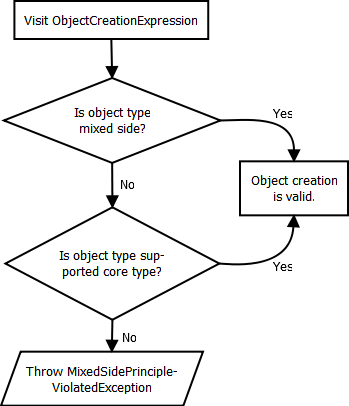
\includegraphics[width=6cm]{resources/images/ValidationFlowchart.png}
		\caption{Deciding whether an object creation is legal when validating methods with the \texttt{MixedSide} attribute}
		\label{fig:isobjectcreationvalid}
	\end{center}
\end{figure}


As the \texttt{AnotherExampleClass} class is also mixed side (it contains a method with the \texttt{MixedSide} attribute) the object creation is legal. If it had not contained any mixed side methods, the object creation would have been illegal and an exception of type \texttt{MixedSidePrincipleViolatedException} had been thrown.

The validation of a member access expression (the access to \newline\texttt{a.AnotherExampleMethod} in Figure~\ref{fig:mixedSideValidationExample}) is done in a very similar way, only checking if the member (in this case, the \texttt{AnotherExampleMethod} method) is a mixed side member, or a supported core type member. 

Even though not shown in the example, it is also important to validate invocations (e.g. method calls) on core types. This is done using the \newline\texttt{VerifyCorrectUseOfSupportedCoreType} method on the \texttt{TypeManager}. This method first checks if the given invocation is done on a core type, and subsequently uses the Core Mapping Specification (as discussed in section \ref{sub:type_mapping}) to verify that we are able to map the invocation to Script\#.
		






	
	% subsection validating (end)
% section syntax_tree_validation (end)